\section{Security in Critical Transport Infrastructures}


\paragraph{Air Traffic Control ATC}
\begin{itemize}
	\item \textbf{Primary Surveillance Radar PSR}:
	ground based, measures time delta between transmission and reflection $\Rightarrow$ independent.
	\item \textbf{Secondary Surveillance Radar SSR}:
	Transponder based interrogation $\Rightarrow$ dependent. \\
	Mode A (identification code), Mode C (identification code + barometric altitude), Mode S (selective addressing to interrogate a specific aircraft, used in \textit{Traffic Alert and Collision Avoidance System})
	\item \textbf{Automatic Dependent Surveillance-Broadcast ADS-B}:
	Aircraft determines its position via satellite and regularly broadcasts the result.
	Replaces functions of SSR, and enables inter-aircraft situational awareness.
\end{itemize}

\paragraph{Problem Statement}
Huge number of systems and protocols in aviation (see \autoref{fig:air-systems}).
None has confidentiality, integrity or authentication.
On the other hand, attacker capabilities grow as domain knowledge spreads and software defined radios become cheaper.
\\
At the same time change is incredibly slow due to certifications and legacy compatibility.

\begin{figure}[h]
	\centering
	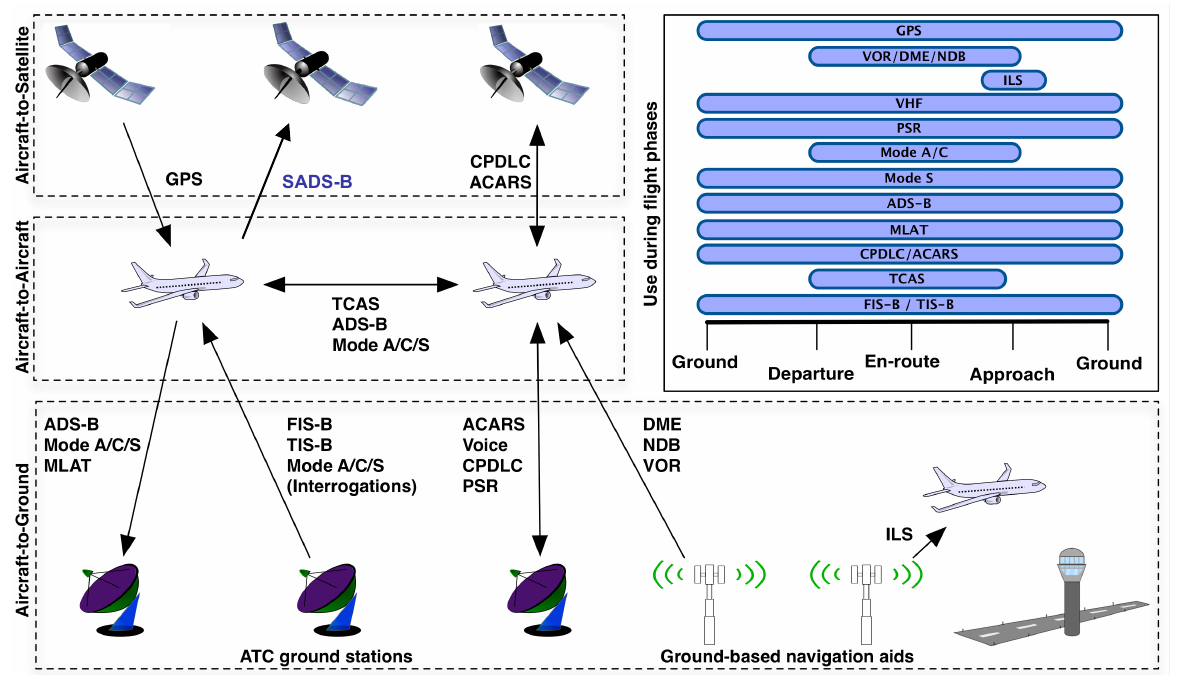
\includegraphics[scale=0.5]{images/6-air-systems.png}
	\caption{Overview of aviation systems}
	\label{fig:air-systems}
\end{figure}



\subsection{Privacy Issues in Aviation}

\paragraph{No confidentiality of aircraft-ground communication}
Clear-text transmission of passenger medical status, forgotten belongings, credit card transaction details, etc.

\paragraph{Proprietary crypto}
ACARS\footnote{Aircraft Communications Addressing and Reporting System}
datalink encryption uses a mono-alphabetic substitution cipher with a limited keyset hardcoded in a lot of private/military/government jets.

\paragraph{Aircraft identifiers}
Aircraft transponders have unique IDs that include aircraft type and operator.
These are not easily and legally changed (unless aircraft is sold).

\paragraph{No location privacy}
Aircraft are globally trackable by anyone.
Either using websites like Flight-Radar24 (heavily filtered), ADS-B Exchange, OpenSky Network.
Or collecting own data from SSR and ADS-B signals using a cheap radio.

\underline{Possible ``uses'' for tracking}:
government aircraft movement, mergers \& acquisitions (M\&A) activities.

\underline{Mitigations:}
Block aircrafts on tracking websites, obscure ownership (register to shell/trust companies), disable position broadcasts (still easily localised near departure/destination airports), use commercial transport.

\subsection{Security Issues in Aviation}

\paragraph{Attacks}
The usual candidates: jamming, modification, injection (ghost aircraft = DoS on ATC).

\paragraph{Safety vs Security}
\textit{Safety} is about dealing with accidents and failures.
We tackle it with experience (root cause analysis) and redundancy (decreasing the likelihood of failure of the entire system).

\textit{Security} on the other hand is concerned with protecting against an intelligent, adaptive attacker.
See the Swiss Cheese model in \autoref{fig:swiss-cheese}.

\begin{figure}[h]
	\centering
	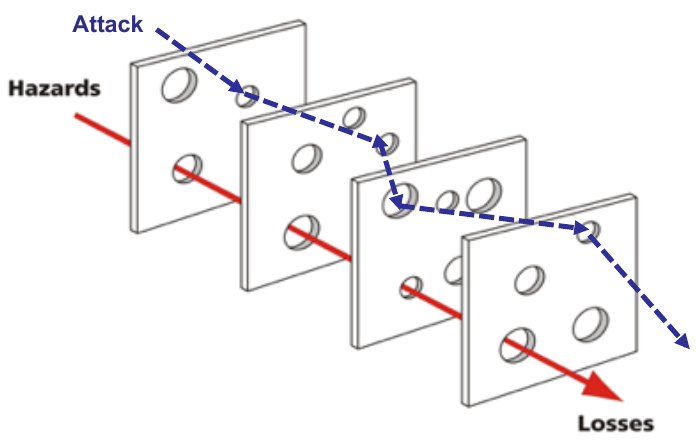
\includegraphics[scale=0.5]{images/6-swiss-cheese.png}
	\caption{Swiss Cheese Model: Safety vs Security}
	\label{fig:swiss-cheese}
\end{figure}

\paragraph{Traffic Collision Avoidance System TCAS}
Aircraft continuously predict each others' paths.
If the paths are too close but not yet at risk, a \textit{traffic advisory TA} is issued (and announced in the cockpit).
If they remain on a close path, a \textit{resolution advisory RA} is announced as compulsory instructions.

\underline{Attack:}
Attacker listens to target aircraft and injects TCAS responses, forcing a TA and RA, thus forcing the aircraft to make unwanted course changes (plus push pilots to reduce TCAS sensitivity).



\subsection{Short-term Security Countermeasures}

\paragraph{Cyber-Physical Countermeasures}
There won't be any real crypto any time soon.
In the meantime, exploit physical layer data (timing, signal strength, Doppler shift, etc) to validate signals.
Throw in some machine learning as well (for anomaly detection).
\\
This hopefully lifts the bar back up to nation-state-attackers-only,

\paragraph{Multilateration}
Use multiple ground stations to receive (and validate) signals from aircraft.

\paragraph{OpenSky Network}
Crowdsources ATC.
Volunteers install software-defined radios around the world to capture signals and publish them.

Short-term solution: rather than cryptographically authenticating messages between aircraft, use ground network to check if everybody else also received the same signal.

\underline{Advantages:}
Does not touch legacy systems, low cost, global coverage, flexible.



\subsection{Satellite and Maritime Infrastructures}

\paragraph{Satellite links}
Signals are receptable in a large area (continent-scale).
This allows tracking of e.g. military aircraft from far away.

\paragraph{Maritime VSAT} (Very Small Aperture Terminal). Still large and expensive.
Connects ships to IP network on land (WiFi, fleet monitoring, weather, navigation, cargo, etc).
Composed of a satellite uplink (large beam, since satellite needs to cover a large area $\Rightarrow$ can be captured from far away) and a directed downlink (towards a ground/land station).
\\
Example: \textit{Electronic Chart Display and Information System ECDIS} (paper chart/map replacement) receives updates via VSAT.

\underline{Analysis:}
Lots of interesting yet unencrypted traffic -- from standard DNS/VoIP/IMAP to specific ``ship data''.

\paragraph{TLDR} It's bad.

